%---------
% place your email id between the braces so that your homework has a name
\def\yourname{}
% -----------------------------------------------------
\def\duedate{5/10/24}
\def\duelocation{via \href{https://www.gradescope.com/courses/753885}{Gradescope}}
\def\hnumber{8}
\def\prof{Lorenzo Orecchia}
\def\course{\href{https://canvas.uchicago.edu/courses/56880}{CMSC 27200 - Spring 2024}}
%-------------------------------------

\documentclass[10pt]{article}
\usepackage[colorlinks,urlcolor=blue]{hyperref}
\usepackage[osf]{mathpazo}
\usepackage{amsmath,amsfonts,graphicx}
\usepackage{latexsym}
\usepackage{subfig}
\usepackage{tkz-graph}
\usepackage{algpseudocode}
\usepackage[shortlabels]{enumitem}
\usepackage{algorithm}
\usepackage{listings}
%\usepackage[top=1in,bottom=1.4in,left=1.5in,right=1.5in,centering]{geometry}
\usepackage{fullpage}
\usepackage{color}
\definecolor{mdb}{rgb}{0.3,0.02,0.02} 
\definecolor{cit}{rgb}{0.05,0.2,0.45}
\usepackage{wrapfig}
\usepackage{graphicx}
%\pagestyle{myheadings}
\markboth{\yourname}{\yourname}

\thispagestyle{empty}

\newenvironment{proof}{\par\noindent{\it Proof.}\hspace*{1em}}{$\Box$\bigskip}
\newcommand{\qed}{$\Box$}
\newcommand{\alg}[1]{\mathsf{#1}}
\newcommand{\handout}{
   \renewcommand{\thepage}{H\hnumber-\arabic{page}}
   \noindent
   \begin{center}
      \vbox{
    \hbox to \columnwidth {\sc{\course} --- \prof \hfill}
    \vspace{-2mm}
    \hbox to \columnwidth {\sc due \MakeLowercase{\duedate} \duelocation\hfill {\Huge\color{mdb}H\hnumber.\yourname}}
      }
   \end{center}
   \vspace*{2mm}
}
\newcommand{\solution}[1]{
\vspace{2mm}

\noindent Collaborators:

\vspace{5mm}

\medskip\noindent{\color{cit}\textbf{Solution:} #1}}

\newcommand{\bit}[1]{\{0,1\}^{ #1 }}
\newcommand{\extraspace}{\medskip\noindent{\color{cit} Extra space for your solution}\newpage}
%\dontprintsemicolon
%\linesnumbered=
\newtheorem{problem}{\sc\color{cit}Problem}
\newtheorem{lemma}{Lemma}
\newtheorem{theorem}{Theorem}
\newtheorem{definition}{Definition}
\newtheorem{claim}{Claim}


\begin{document}
\handout
\begin{itemize}
\item The assignment is due at Gradescope on \duedate.

\item A LaTeX template will be provided for each homework. You are strongly encouraged to type your homework into this template using \LaTeX.  If you are writing by hand, please fill in the solutions in this template, inserting additional sheets as necessary. This will help facilitate the grading.

\item You are permitted to discuss the problems with up to 2 other students in the class (per problem); however, {\em you must write up your own solutions, in your own words}. Do not submit anything you cannot explain. If you do collaborate with any of the other students on any problem, please list all your collaborators in the appropriate spaces.

\item Similarly, please list any other source you have used for each problem, including other textbooks or websites.

\item {\em Show your work.} Answers without justification will be given little credit.

\item Your homework is \textit{resubmittable}. Please refer to the course syllabus on Canvas for a more detailed description of this. For any problem that you have not changed from your last submission, please make sure to indicate this in your submission to help our graders grade faster. 

\end{itemize}

\newpage

%%%%%%%%%%%%%%%%%%%%%%%%%%%%%%%%%%%%%%%%%%%

%%%%%%%%%%%%%%%%%%%%%%%%%%%%%%%%%%%%%%%%%%%

\begin{problem}[Knapsack and Linear Programs]
Recall the 0-1 Knapsack problem discussed in class: we are given a set of items with values and weights: $\{(v_i,w_i)\}_{i=1}^n$ and a weight budget $W$, and we are interested in finding the choice of items (i.e. the subset $S$ of $[n]$) maximizing the sum of the values of the items:
\[
    \sum_{i\in S} v_i,
\]
subject to the weight constraints:
\[
    \sum_{i\in S} w_i < W.
\]
Consider the following linear program:
\begin{align}\label{LP}
    \max_{x \in \mathbb{R}^n} \quad &\sum_{i\in [n]}x_iv_i\\
    &  \sum_{i\in [n]}x_i w_i \leq W \nonumber \\
    & 0 \leq x_i \leq 1 \hspace{1cm} \forall i\in [n]\nonumber 
\end{align}
Here, each variable $x_i$ is meant to indicate whether or not we are including a specific item in our solution.
\begin{enumerate}[(a)]
    \item Explain why the above linear program (\ref{LP}) doesn't solve the original 0-1 Knapsack problem, and provide an example instance of the 0-1 Knapsack problem that this LP gives an invalid solution for. 
    \item Describe the problem, in words, that is solved by an instance of (\ref{LP}).
    \item Describe (in words) and give the pseudocode of an algorithm that finds the optimal assignment of $x$ in (\ref{LP}).
    \item Compute the dual of (\ref{LP}).
\end{enumerate}

\end{problem}

\begin{solution}

\begin{enumerate}[(a)]

    \item {
        (\ref{LP}) optimizes over $[0,1]^n$, which is continuous. 
        We want solutions that are binary. 

        We could map solutions in $[0,1]^n$ to $\{0, 1\}^n$ by 
        rounding. 
        However, the optimum in continuity is not necessarily optimal in binary 
        after rounding. 

        Consider, for example, the instantiation of (\ref{LP}) with 
        $n=2$, $v = \{1, 0.2\}$, $w = \{8, 2\}$, and $W = 3$. 
        The feasible region is:

        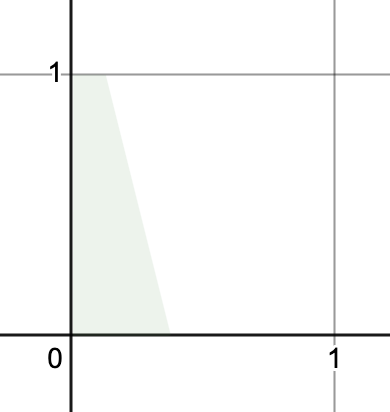
\includegraphics[scale=0.5]{1}

        \textit{Note: $x_1$ and $x_2$ correspond to the $x$ and $y$ axes, respectively.} 

        (\ref{LP}) gives $x_1=0.375$, $x_2=0$ as the optimum. 
        Rounding up gives infeasible points, and rounding down gives 
        $x_1=0$, $x_2=0$. 

        The true optimum, however, is $x_1=0$, $x_2=1$. 
    }
    \item {
        (\ref{LP}) solves the knapsack problem for non-quantized, continous 
        items. 

        For example, Antares is at $7/11$ and wants an ICEE. 

        There are $n$ flavors, and each flavor $i$ costs $w_i$ dollars per ounce 
        and gives Antares $v_i$ units of enjoyment per ounce. 
        Unfortunately, the ICEE machine is broken and can dispense at most $1$ 
        ounce of each flavor. 
        On the bright side, however, it is the future and money is continuous! 

        If Antares only has $W$ dollars, how much of each flavor should he get 
        to maximize enjoyment?
    }
    \item {
    
        We could solve this LP by simplex. 
        However, because solutions can take continuous values, a greedy 
        algorithm presents itself naturally. 

        To get an optimal 'knapsack', we simply take as much of the most value 
        efficent items as we can. 

        \begin{algorithm}[H]
            \caption{Greedy Algorithm for the Continuous $0$-$1$ Knapsack Problem}
            \begin{algorithmic}[1]

                \Statex \textbf{Input: } $n, v_i, w_i, W$
                \Statex \textbf{Output: } $K : i \rightarrow \mathbb{R}[0, 1]$

                \State $I \gets \{1, \dots, n\}.sort(\text{key}=\frac{v_i}{w_i})$

                \State $K \gets []$

                \For{$i \in I$}
                    \State \textbf{if $w_i < W$ do} 
                    \State \qquad $K[i] \gets 1$
                    \State \qquad $W \gets W - w_i$
                    \State \textbf{else do}
                    \State \qquad $K[i] \gets \frac{W}{w_i}$
                    \State \qquad \textbf{break}
                \EndFor

                \State \textbf{return $K$}

            \end{algorithmic}
        \end{algorithm}
    }
    \item {
        The primal LP is expressed as:
        \begin{align*}
            \max_{\vec{x}} \vec{x} \cdot \vec{v} \\
            \vec{x} \cdot \vec{w} \leq W \\
            0 \leq \vec{x} \leq 1
        \end{align*}
        The implied constraint is:
        \begin{align*}
            \lambda_w \vec{x} \cdot \vec{w} + \lambda_1 x_1 + \dots + \lambda_n x_n \leq \lambda_w W + \sum_{i=1}^n \lambda_i \\
            \sum_{i=1}^n (\lambda_w w_i + \lambda_i)x_i \leq \lambda_w W + \sum_{i=1}^n \lambda_i
        \end{align*}
        To create our bound on the primal, we use $\vec{x} \geq 0$ to say:
        \begin{align*}
            \lambda_w w_i + \lambda_i \geq v_i
        \end{align*}
        The dual is then:
        \begin{align*}
            \min_{\lambda_i, \lambda_w} [\lambda_w W + \sum_{i=1}^n \lambda_i] \\
            \lambda_w w_i + \lambda_i \geq v_i \\
            \lambda_w, \lambda_i \geq 0
        \end{align*}

    }

\end{enumerate}

\end{solution}

\newpage
%%%%%%%%%%%%%%%%%%%%%%%%%%%%%%%%%%%%%%%%%%%

%%%%%%%%%%%%%%%%%%%%%%%%%%%%%%%%%%%%%%%%%%%
\begin{problem}[Bottleneck and Lower-Binding Edges]
Let $G$ be a flow network with integer edge capacities. An edge in $G$ is upper-binding if increasing its capacity by 1 also increases the value of the maximum flow in $G$. Similarly, an edge is lower-binding if decreasing its capacity by 1 also decreases the value of the maximum flow in $G$.
\begin{enumerate}[(a)]
    \item Does every flow network G have at least one upper-binding edge? If so, sketch a proof. If not, give a counterexample.
    \item Does every flow network G have at least one lower-binding edge? If so, sketch a proof. If not, give a counterexample.
    \item Recall that an edge is saturated under a flow f if $f(e) = c(e)$. Prove or disprove: Given a flow network $G$, if an edge $e$ is saturated under a max flow $f$, then $e$ is an upper-binding edge.
    \item Given a flow $f$ on a flow network, we define the divergence $div(v)$ at a vertex as:
    \[
        \sum_{(v,u)\in E} f_{vu} - \sum_{(w,v) \in E} f_{wv}.
    \]
    
    Sketch a proof that given any subset $S \subseteq V$:
    \[
        \sum_{v \in S} div(v) = \sum_{(u,v) \in E(S,\overline{S})} f_{uv} - \sum_{(u,v) \in E(\overline{S},S)} f_{uv},
    \]
    i.e. the total amount of flow out of $S$ minus the total amount of flow into of $S$ is equal to the total divergence inside of $S$.
    
    
    (This is a discrete version of what is known as the divergence theorem in multivariable calculus, though understanding this is not needed to solve this problem).
    \item Formally prove the following statement: Given a flow network $G$, if an edge $e$ is an upper-binding edge, then $e$ is saturated under \textbf{any} max flow $f$.
\end{enumerate}
\end{problem}

\begin{solution}

\begin{enumerate} [(a)]
    
    \item {

        Consider the flow network:

        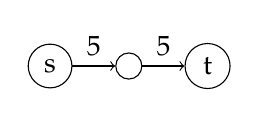
\begin{tikzpicture}
            \node[shape=circle,draw=black] (s) {s};
            \node[shape=circle,draw=black] (v) [right of=s] {};
            \node[shape=circle,draw=black] (t) [right of=v] {t};

            \path [->] (s) edge node[above] {$5$} (v);
            \path [->] (v) edge node[above] {$5$} (t);
        \end{tikzpicture}

        There is no upper-binding edge because both:

        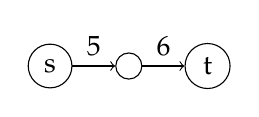
\begin{tikzpicture}
            \node[shape=circle,draw=black] (s) {s};
            \node[shape=circle,draw=black] (v) [right of=s] {};
            \node[shape=circle,draw=black] (t) [right of=v] {t};

            \path [->] (s) edge node[above] {$5$} (v);
            \path [->] (v) edge node[above] {$6$} (t);
        \end{tikzpicture}
        \qquad \qquad
        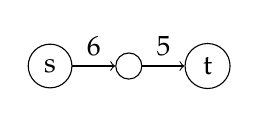
\begin{tikzpicture}
            \node[shape=circle,draw=black] (s) {s};
            \node[shape=circle,draw=black] (v) [right of=s] {};
            \node[shape=circle,draw=black] (t) [right of=v] {t};

            \path [->] (s) edge node[above] {$6$} (v);
            \path [->] (v) edge node[above] {$5$} (t);
        \end{tikzpicture}

        still have max-flow $5$. 

    }
    \item {
        According to the max-flow min-cut theorem, the size of the max flow in G 
        equals the capacity of the smallest $(s, t)$ cut. 

        Then decreasing the capacity of the cut at any edge will necessarily 
        decrease the maximum flow in $G$, as all flow must pass through the cut. 
    }
    \item {
        This statement is false. 
        Consider again the counter example:

        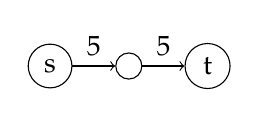
\begin{tikzpicture}
            \node[shape=circle,draw=black] (s) {s};
            \node[shape=circle,draw=black] (v) [right of=s] {};
            \node[shape=circle,draw=black] (t) [right of=v] {t};

            \path [->] (s) edge node[above] {$5$} (v);
            \path [->] (v) edge node[above] {$5$} (t);
        \end{tikzpicture}

        The max-flow here is $5$, so both edges are saturated. 
        However, no upper-binding edge exists. 
    }
    \item {
        Let $(u, v)$ denote any internal edge of $S$ such that $u, v \in S$. 
        
        When computing:
        $$
        \sum_{v \in S} div(v)
        $$
        $(u, v)$ and $(v, u)$ cancel out because $(u, v)$ is added while doing
        $div(u)$ but subtracted when $div(v)$. 
        It holds that all interal edges are canceled out in this way. 
        
        Thus, the only edges not canceled in the sum are those that involve some 
        edge outside $S$. 
        The right hand side computes the amount of flow carried by these 
        external edges. 
    }
    \item {
        Let $e$ be an upper-binding edge. 
        Suppose $e$ is not saturated under some max flow $f$. 
        This implies some bottleneck upstream or downstream is limiting the flow 
        through $e$. 
        Thus, increasing the capacity of $e$ will not increase the max-flow 
        because the bottlenecks still exist. 
        But then $e$ is not an upper-binding edge, contradicting our assumption. 
    }

\end{enumerate}

\end{solution}

\newpage


%%%%%%%%%%%%%%%%%%%%%%%%%%%%%%%%%%%%%%%%%%%

%%%%%%%%%%%%%%%%%%%%%%%%%%%%%%%%%%%%%%%%%%%
\begin{problem}[A Flowy Metric]
Consider an undirected graph $G = (V, E)$ with capacities $c_e\ge 0$ on all edges $e \in E$. $G$ has property that any cut in $G$ has capacity at least $1$. For example, a graph with a capacity of $1$ on all edges is connected if and only if all cuts have capacity at least $1$. However, in our case, $c_e$ can be any non-negative number.
\begin{enumerate}[(a)]
    \item Show that for any two vertices $s, t \in V$, the max flow from $s$ to $t$ is at least $1$.
    \item Define the \textbf{length} of a flow $f$ to be $\texttt{length}(f) = \sum_{e\in E} |f_e|$. Define the \textbf{flow distance} $d_{\text{flow}} (s,t)$ to be the minimum length of any $s$-$t$ flow $f$ that sends one unit of flow from $s$ to $t$ and satisfies all capacity constraints (i.e. $|f_e|\le c_e$ for all $e \in E$). Write an LP that computes $d_{\text{flow}} (s,t)$. 
    \item Prove that if $c_e = 1$ for all $e\in E$, then $d_{\text{flow}} (s,t)$ is the length of the shortest path in $G$ from $s$ to $t$. \\
    (Hint: let $d(s,t)$ be the length of the shortest path from $s$ to $t$. You want to show $d_{\text{flow}} (s,t) = d(s,t)$ which is equivalent to showing that $d_{\text{flow}} (s,t) \le d(s,t)$ and $d_{\text{flow}} (s,t) \ge d(s,t)$.)
\end{enumerate}
\end{problem}

\begin{solution}

\begin{enumerate}[(a)]
    \item {
        Max-flow min-cut says that the max flow for any $s$ and $t$ is the 
        capacity of the smallest $(s, t)$ cut. 

        If the capacity of all cuts are $\geq 1$, then the smallest $(s, t)$ cut 
        must have capacity $\geq 1$. 
        Thus, the max flow is $\geq 1$. 
    }
    \item {
        LP:
        \begin{align*}
            & \min \sum_{e \in E} f_e \\
            & \sum_{(s, v) \in E} f_v = 1 \\
            & \sum_{(u, v) \in E'}f_{uv} = \sum_{(v, w) \in E'}f_{vw} 
            \quad \forall u \neq s \quad \forall w \neq t \\
            & 0 \leq f_e \leq c_e \\
        \end{align*}
    }
    \item {
        Let $d(s, t)$ be the length of the shortest path $P$ from $s$ to $t$. 

        Consider the flow $f$ associated with $d_{flow}(s, t)$. 
        It sends $1$ unit of flow from $s$ to $t$. 
        Thus, by flow conservation, no $f_e > 1$. 
        Moreover, since $f$ must be minimal in length, we can immediately 
        propose a solution to $f$ that sends $1$ unit of flow along $P$. 
        $d(s, t)$ thus bounds $d_{flow}(s, t)$ from above. 

        However, $d_{flow}(s, t)$ must be at least $d(s, t)$. 
        It cannot be $< d(s, t)$, which would imply the flow travels along some 
        path shorter than $P$, contradicting our assumption that $P$ is optimal. 

        Thus, $d_{flow}(s, t) = d(s, t)$. 
    }
\end{enumerate}

\end{solution}


\newpage

%%%%%%%%%%%%%%%%%%%%%%%%%%%%%%%%%%%%%%%%%%%

%%%%%%%%%%%%%%%%%%%%%%%%%%%%%%%%%%%%%%%%%%%
\begin{problem}[Road Trip 4: Road Trip Game] Lorenzo is going on another trip, and he's taking Ruimin along with him. They've already figured out the shortest path to take, and the optimal gas stations to stop at along the way - all they need left is some entertainment. Thankfully, Lorenzo has thought of a great game to keep them entertained.  

The game is specified by an undirected, unweighted graph $G=(V,E)$ and two vertices $s,t\in V$. Lorenzo picks an edge $e \in E$, and Ruimin simultaneously picks a cut $S \subseteq V$ which must separate $s$ and $t$ i.e. $s \in S$ but $t \not\in S$. We define the edge boundary of a cut $S$ to be the set of edges crossing the cut:
\[
    E(S,\overline{S}) := \{uv \in E \mid u \in S, v \in \overline{S}\}.
\]

\noindent
Lorenzo wins the game if the edge he picked is in Ruimin's cut's edge boundary, and Ruimin wins otherwise. Formally, for the selected $e$ and $S$, Lorenzo's payoff $P(e, S)$ is given by
\[
    P(e,S) = \begin{cases} 1 & \text{if } e\in E(S,\overline{S}),\\
    0 & \text{otherwise.}\end{cases}
\]
Lorenzo is trying to maximize $P(e, S)$, and Ruimin is trying to minimize it. 

\noindent
We are interested in \textbf{mixed strategies} for this game: Lorenzo will assign each edge $e$ some probability $p_e \geq 0$, and randomly select an edge accordingly. Similarly, Ruimin's strategy will involve randomly selecting a cut $c$, where each cut $c$ is selected with probability $p_c$.

\begin{enumerate}[(a)]
    \item Lorenzo knows that he can't outsmart Ruimin, so he knows that whatever strategy he picks, Ruimin is just going to read his mind and figure it out. To determine his best strategy, he is going to solve the following LP:
    \begin{align*}
        \max_{\alpha, q}\quad& \alpha \\
        &  \sum_{e \in C} q_e \geq \alpha  \hspace{0.5cm} \forall C \in \mathcal{C}\\
        & \sum_e q_e = 1\\
        & 0 \leq q_e  \hspace{0.5cm} \forall e \in E(G)
    \end{align*}
    where $\mathcal{C}$ is the set of s-t cuts in $G$. Explain, in words, how this LP represents the game. 
    \item Ruimin knows that Lorenzo is a cheater, so he knows that whatever strategy he picks, Lorenzo is going to sneakily take a glance at it before deciding on his own strategy. In that case, write the linear program that Ruimin must solve to determine his optimal strategy. (Assume that Lorenzo picks his strategy after Ruimin.)
    \item Demonstrate that these programs are each other's dual. (You may use the fact that the dual of a dual program is the primal.)
    \item Part (c) implies the existence of some probability $p$ such that:
    \begin{itemize}
        \item If Lorenzo plays optimally, his probability of winning is at least $p$, even if Ruimin knows his strategy.
        \item If Ruimin plays optimally, Lorenzo's probability of winning is at most $p$, even if Lorenzo knows Ruimin's strategy.
    \end{itemize}
    Provide a short argument (2 sentences) that part (c) implies this. 
    \item Sketch a proof that the $p$ from part (d) is $p=\frac{1}{L}$ where $L$ is the length of a shortest path from $s$ to $t$. This is Lorenzo's expected payoff from the game if both players play optimally, and is known as the \textbf{value} of the game. 
\end{enumerate}
\end{problem}

\begin{solution}

\begin{enumerate}[(a)]
    \item {
        The constraints $\sum_e q_e = 1$ and $0 \leq q_e$ ensure $q$ is a valid 
        probability distribution over the edges, enforcing non-negativity and 
        unit measure, respectively.  

        The constraint $\sum_{e \in C} q_e \geq \alpha$ for all $C$ defines 
        $\alpha$ as a lower bound on the probability of choosing an edge in a 
        cut $C$. 

        By maximizing $\alpha$, Lorenzo finds a distribution over which he has 
        the best chance of selecting any given cut. 

        Since Ruimin can read Lorenzo's mind, this strategy ensures that no 
        matter which cut Ruimin selects, Lorenzo will have some chance at 
        winning. 
    }
    \item {
        LP to minimize Lorenzo's chance of winning:
        \begin{align*}
            \min_{\alpha, C} \alpha \\
            p_c \geq \alpha \quad \forall c \in \mathcal{C} \\
        \end{align*}
    }
    \item {
        The primal:
        \begin{align*}
            \max_{\alpha, q} \alpha \\
            \sum_{e \in C} q_e \geq \alpha  \quad \forall C \in \mathcal{C} \\
            \sum_e q_e = 1 \\
            0 \leq q_e  \quad \forall e \in E(G)
        \end{align*}
        Implied constraint:
        \begin{align*}
            \lambda \sum_e q_e + 
            \sum_{C \in \mathcal{C}} \lambda_C \sum_{e \in C} q_e \geq
            \lambda + \alpha \sum_{C \in \mathcal{C}} \lambda_C \\
        \end{align*}
        Since $q_e \geq 0$:
        \begin{align*}
            \lambda + \sum_{C \in \mathcal{C}} \lambda_C \: \mathbb{1}[e \in C] \geq 0
        \end{align*}
        Since $\alpha \geq 0$:
        \begin{align*}
            \sum_{C \in \mathcal{C}} \lambda_C \geq 1
        \end{align*}
    }
\end{enumerate}

\end{solution}


\end{document}